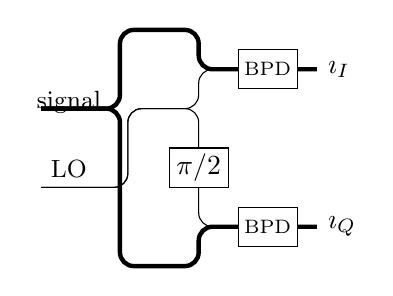
\begin{tikzpicture}
    \draw[rounded corners=5pt, ultra thick] (0,0)node[above right = -2mm]{\small signal} --++ (1,0) --++ (0,1) --++ (1,0) --++ (0,-0.5) --++ (0.5,0)--++ (1,0) node[right]{$\imath_I$};
    \draw[rounded corners=5pt, ultra thick] (0,0) --++ (1,0) --++ (0,-2) --++ (1,0) --++ (0,+0.5) --++ (0.5,0)--++ (1,0) node[right]{$\imath_Q$};

    \draw[rounded corners=5pt] (0,-1)node[above right]{\small LO} --++ (1.1,0) --++ (0,+1) --++ (0.9,0) --++ (0,+0.5) --++ (0.25,0);
    \draw[rounded corners=5pt] (0,-1) --++ (1.1,0) --++ (0,+1) --++ (0.9,0) --++ (0,-1.5)  --++ (0.25,0);

    \draw[fill = white] (2.5,0.25) rectangle (3.25,0.75)node[midway]{\scriptsize BPD};
    \draw[fill = white] (2.5,-1.75) rectangle (3.25,-1.25)node[midway]{\scriptsize BPD};
    \draw[fill = white] (1.625,-1) rectangle (2.375,-0.5)node[midway]{$\pi/2$};
\end{tikzpicture}
